\documentclass[a4paper]{article}
\usepackage[utf8]{inputenc}
\usepackage[russian,english]{babel}
\usepackage[T2A]{fontenc}
\usepackage[left=10mm, top=20mm, right=18mm, bottom=15mm, footskip=10mm]{geometry}
\usepackage{indentfirst}
\usepackage{amsmath,amssymb}
\usepackage[italicdiff]{physics}
\usepackage{graphicx}
\graphicspath{{images/}}
\DeclareGraphicsExtensions{.pdf,.png,.jpg}
\usepackage{wrapfig}

\usepackage{caption}
\captionsetup[figure]{name=Рисунок}
\captionsetup[table]{name=Таблица}
  
\title{\underline{Отчет о выполненой лабораторной работе 1.2.5}}
\author{Воронин Денис, Б04-403}



\begin{document}

\maketitle
\begin{center}
    \textbf{Исследование вынужденной регулярной процессии гироскопа}
\end{center}

\section{Аннотация}
\textbf{Цель работы:}  исследовать вынужденную прецессию гироскопа, установить зависимость скорости вынужденной прецессии от величины момента сил, действующий на ось гироскопа и сравнить ее со скоростью, рассчитанной по скорости прецессии.\par

\textbf{В работе используются:}гироскоп в кардановом подвесе, секундомер, набор грузов, отдельный ротор гироскопа, цилиндр известной массы, крутильный маятник, штангенсциркуль, линейка.\par
	
\section{Теоретические сведения}

Момент импульса твердого тела в 3-х его ллавных осях x, y, z равен
\[\overrightarrow{L} = \overrightarrow{i}I_{x}\omega_{x} + \overrightarrow{j}I_{y}\omega_{y} + \overrightarrow{k}I_{z}\omega_{z}\] 
где $I_{x}, I_{y}, I_{z}$ - главные моменты инерции, $\omega_{x},\omega_{y},\omega_{z}$ - компоненты вектора угловой скорости $\overrightarrow{\omega}$. Быстро вращающееся тело, для которого, например, 
\[I_{z}\omega_{z} \gg  I_{x}\omega_{x}, I_{y}\omega_{y}\]
Принято называть гироскопом. Гироскоп называется уравновешанным, если его центр масс неподвижен. \par
В силу $\frac{d\overrightarrow{L} }{dt} = \overrightarrow{M}  $ приращение момента импулься определяется интеграллом
\[\bigtriangleup \overrightarrow{L} = \int\overrightarrow{M}dt (1)\] 

\begin{wrapfigure}{r}{0.5\textwidth}
    \centering
    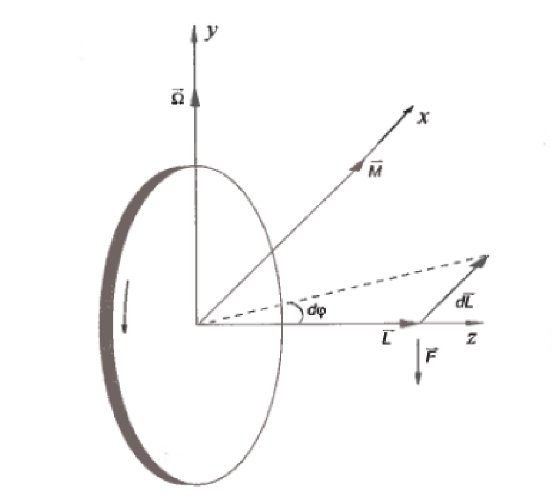
\includegraphics[width=0.4\textwidth]{pick1.PNG}
    \caption{Маховик}
\end{wrapfigure}

Если момент внешних сил действует в течение короткого промежутка времени, из интеграла (1) следует, что приращение $\bigtriangleup \overrightarrow{L} $  момента импульса значительно меньше самого момента импульса:
\[\left\lvert\bigtriangleup \overrightarrow{L} \right\rvert \ll \left\lvert \overrightarrow{L} \right\rvert  \]
С этим связана замечательная устойчивость, которую приобретает дви- жение гироскопа после приведения его в быстрое вращение.\par

Выясним, какие силы надо приложить к гироскопу, чтобы изменить направление его оси. Рассмотрим для примера маховик, вращающийся вокруг оси z, перпендикулярной к плоскости маховика (рис. 1). Будем считать, что


\[\omega_{z} = \omega_{0} , \omega_{x} = \omega_{0}, \omega_{y} = \omega_{0}\]

Пусть ось вращения повернулась в плоскости zx по направлению к оси х на бесконечно малый угол dy. Такой поворот означает добавочное враще- ние маховика вокруг оси у, так что
\[d\varphi  = \Omega dt \]
где $\Omega $- угловая скорость такого вращения. Будем предполагать, что 
\[L_{\Omega }\ll L_{\omega_{0}}\] \newpage

Это означает, что момент импульса маховика,
равный $I_{z}\omega _{0}$ до приложения внешних сил, только повернется в плоскости zx По направлению к оси х не изменяя своей величины. Таким образом,
\[\left\lvert d\overrightarrow{L} \right\rvert = Ld\varphi  = L\Omega dt\]

Но это изменение направлено вдоль оси х, поэтому вектор $d\overrightarrow{L} $ можно представить в виде векторного произведения вектора угловой скорости $\overrightarrow{\Omega } $, направленного вдоль оси у, на вектор собственного момента
импульса маховика, направленного вдоль оси z,
\[d\overrightarrow{L} = \overrightarrow{\Omega } \times  \overrightarrow{L}dt\]
т.е
\[\frac{d\overrightarrow{L}}{dt} = \overrightarrow{\Omega } \times \overrightarrow{L}\]

Для гироскопа массой $m_{\text{г}}$, у которого ось собственного вращения наклонена на угол $\alpha $ от вертикали, скорость прецессии, происходящей вокруг вертикальной оси под действием силы тяжести, равна

\[\Omega = \frac{M}{I_{z}\omega _{0}\sin \alpha } = \frac{m_{\text{г}}gl_{\text{ц}}\sin \alpha}{I_{z}\omega _{0}\sin \alpha } = \frac{m_{\text{г}}gl_{\text{ц}}}{I_{z}\omega_{0}} \]

где $l_{\text{ц}}$ - расстояние от точки подвеса до центра масс гироскопа, т.е скорость прецессии не зависит от угра $\alpha $ \par

Для изучения регулярной прецессии уравновешанного гироскопа к его оси подвешивают дополнительные грузы.
Это смещает общий центр масс и создает момент сил тяжести, вызывающий прецессию. Скорость прецессии в этом случае равна 
\[\Omega = \frac{mgl}{I_{z}\omega_{0}} \]

Период крутильных колебаний $T_{0}$ зависит от момента инерции $I_{0}$ и модуля кручения проволоки f:
\[T_{0} = 2\pi \sqrt{\frac{L_{0}}{f} }\]

Для определения момента инерции ротора гироскопа имеем
\[I_{0} = I_{\text{ц}}\frac{T_{0}^2}{T_{\text{ц}}^2} \]


\section{Экспериментальная установка}

\begin{wrapfigure}{r}{0.5\textwidth}
    \centering
    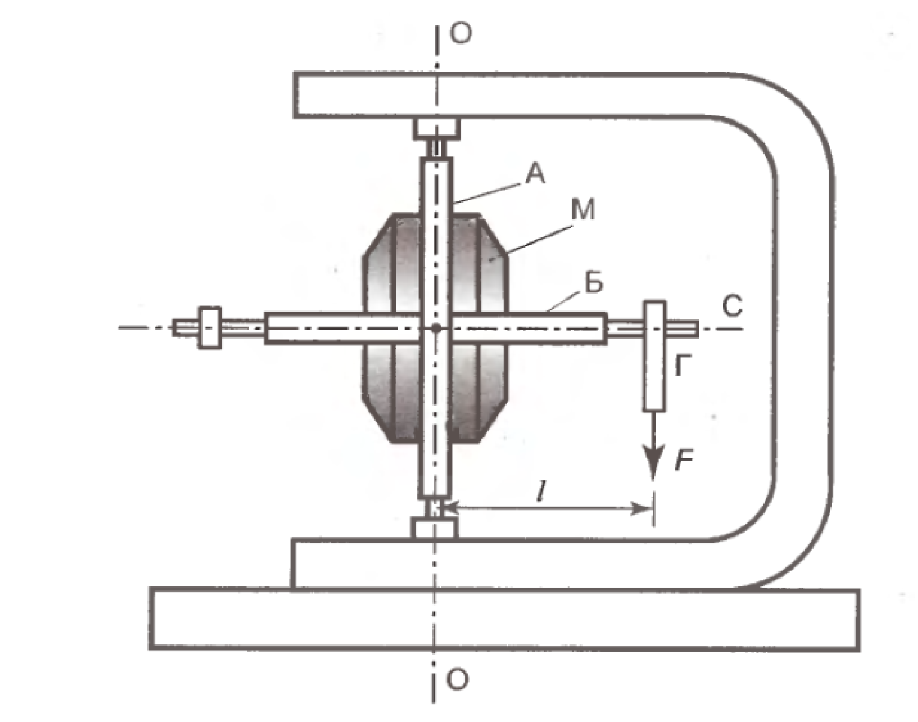
\includegraphics[width=0.5\textwidth]{pick2.PNG}
    \caption{Схема экспериментальной установки}
\end{wrapfigure}

Экспериментальная установка для исследования прецессии уравновешенного гироскопа показана на рис. 2. Ротором гироскопа является ротор высокооборотного электромотора М, питающегося током частотой 400 Гц. Кожух мотора (статор, имеющий обмотки, питаемые током частотой 400 Гц) скреплен с кольцом Б (рис. 2). 
Мотор с кольцом Б может вращаться в кольце А вокруг горизонтальной оси бб, которое может вращаться вокруг вертикальной оси аа. Ротор электромотора представляет массивный стальной цилиндр с прожилками меди, образующими "беличье колесо". Обозначенный на рис. 2 буквой С рычаг направлен по оси симметрии ротора. На рычаг подвешивают грузы Г. Подвешивая различные грузы, можно менять силу F, момент которой определяется расстоянием 1 от точки подвеса до горизонтальной оси кольца А (до центра масс гироскопа), указанным на самой установке.
\newpage
\section{Ход работы}

\subsection{Составление таблиц}

\begin{table}[!h]
    \begin{center}
    \begin{tabular}{|l|l|l|l|}
    \hline
            & Масса, г & Радиус, см & Период, с \\ \hline
    Цилиндр & 1616,3   & 3,9        & 3,97      \\ \hline
    Ротор   & 1083     & 3,4        & 3,17      \\ \hline
    \end{tabular}
    \caption{Данные полученные для расчета момента инерции ротора с помощью цилиндра}
    \end{center}
    \end{table}
l = 121 мм = 0,121 м
\begin{table}[!h]
    \begin{center}
    \begin{tabular}{|l|l|l|l|l|l|}
    \hline
        & Масса груза, г &Момент сил, Н & Время прецессии, с & Угол поворота & Средний период оборащения\\ \hline
    №1& 179               & 0,22          & 232          &1449        &57,62      \\ \hline
      &                   &              & 229           &1446  \\ \hline
      &                &                 & 230           &1458  \\ \hline
    №2& 220            & 0,27           & 205           &1566         & 47,14 \\ \hline
      &                &                 & 207           &1576  \\ \hline
    №3&274             & 0,33           & 165           &1562         & 38,01 \\ \hline
      &                &                 & 164           &1566  \\ \hline
    №4&342             & 0,41           & 156           &1852         & 30,42 \\ \hline
      &                &                 & 166           &1945  \\ \hline
    №5&57              & 0,07           & 179           &360          & 179 \\ \hline
    №5&76              & 0,09           & 133           &360          & 133 \\ \hline
    №6&93              & 0,11           & 109           &360          & 109 \\ \hline
    №7&117             & 0,14           & 87            &360          & 87 \\ \hline
    \end{tabular}
    \caption{Данные для измерения прецессии, зависимость угла поворота от момента сил}
    \end{center}
    \end{table}

Погрешность:
    \[\sigma_{\text{случ}} = \sqrt{\frac{1}{5 \cdot 4}\sum\limits_{i=1}^{5} (\overline{\Omega_{i}} - \Omega_{i})^2}\]
    \[\sigma_{\text{сист}} = \Omega \cdot \varepsilon_{T}\]
    \[\sigma_{\text{полн}} = \sqrt{\sigma_{\text{случ}}^2 + \sigma_{\text{сист}}^2}\]
    

Для удобства в построении графика сделаем отдельную таблицу:

\begin{table}[!h]
    \begin{center}
    \begin{tabular}{|c|c|c|c|}
    \hline
       & Масса груза, $m$, г & Угловая скорость рецессии, $\Omega$, $c{^-1}$ & Момент силы, $M$, Н $\cdot$ м \\ \hline
    №1 & 179                  & 0,101 $\pm$ 0,00012                                     & 0,22                                                                 \\ \hline
    №2 & 220                 & 0,133  $\pm$ 0,0003                                   & 0,27                                                                 \\ \hline
    №3 & 274                 & 0,165  $\pm$ 0,0004                                     & 0,33                                                                   \\ \hline
    №4 & 342                 & 0,206  $\pm$ 0,00055                                      & 0,41                                                                 \\ \hline
    №5 & 57                 & 0,035 $\pm$ 0,0018                                      & 0,07                                                                   \\ \hline
    №6 & 76                 & 0,047 $\pm$ 0,0011                                      & 0,09                                                                   \\ \hline
    №7 & 93                 & 0,058 $\pm$ 0,0028                                      & 0,11                                                                   \\ \hline
    №8 & 117                 & 0,072 $\pm$ 0,0009                                      & 0,14                                                                   \\ \hline

    \end{tabular}
    \caption{Данные для построения графика}
    \end{center}
    \end{table}
\newpage


\begin{figure}[h!]
    \centering
    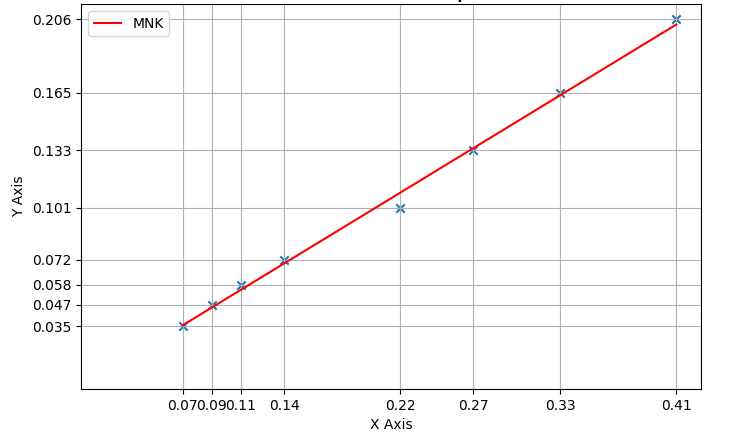
\includegraphics[width=1\textwidth]{pick3}
    \caption{График зависимости угловой скорости рецессии $\Omega$ от момента силы $M$}
\end{figure}


\subsection{Нахождение момента инерции ротора}
Используя данные таблицы 1 и формулу \label{moment} получаем:
\[I_{\text{ц}} = \frac{m_{\text{ц}}R^2}{2} = (123 \pm 1,23) \cdot 10^{-5} \text{ кг}\cdot\text{м}^2 (\varepsilon_{I_{\text{ц}}} = 1\%)\]
\[I_{0} = I_{\text{ц}} \cdot \frac{T_{0}^2}{T_{\text{ц}}^2} = (7,84 \pm 0,067) \cdot 10^{-4} \text{ кг}\cdot\text{м}^2 (\varepsilon_{I_{0}} = 0,8\%)\]
\subsection{Момент силы трения}
	
	Оценить момент силы трения мы можем по формуле: $M = \omega I_0 \omega_0$, а $\sigma_M = M\cdot\sqrt{\varepsilon_M^2+ \varepsilon_k^2}$. Для каждой массы момент силы трения будет свой:
	
	\begin{itemize}
		\item $m = 342$ г, $\omega = 11,71\cdot 10^{-4}$ $\text{с}^{-1}$, $M = (2,21\pm0,02)\cdot10^{-3}$ Н$\cdot$м
		\item $m = 274$ г, $\omega = 11,22\cdot 10^{-4}$ $\text{с}^{-1}$, $M = (2,11\pm0,02)\cdot10^{-3}$ Н$\cdot$м
		\item $m = 220$ г, $\omega = 11,13\cdot 10^{-4}$ $\text{с}^{-1}$, $M = (2,09\pm0,02)\cdot10^{-3}$ Н$\cdot$м
		\item $m = 179$ г, $\omega = 9,04\cdot 10^{-4}$ $\text{с}^{-1}$, $M = (1,70\pm 0,02)\cdot10^{-3}$ Н$\cdot$м
		\item $m = 117$ г, $\omega = 9,55\cdot 10^{-4}$ $\text{с}^{-1}$, $M = (1,65 \pm 0,02)\cdot10^{-3}$ Н$\cdot$м
	\end{itemize} 

\subsection{Нахождение частоты вращения ротора гироскопа}

Частота вращения будет равна $\omega_{0} = \frac{1}{kI_{0}}$, где $k$ - угол наклона прямой графика $\Omega(M)$
Из графика $k = 0,49$

Получаем $\omega_{0} = 2493,1 \text{ с}^{-1}$

Погрешность $\sigma_{\omega_{0}} = \omega_{0} \cdot \varepsilon_{I_{0}} \approx 17,96 \text{ с}^{-1} (\varepsilon_{\omega_{0}} = 0,8\%)$

Отсюда частота вращения ротора гироскопа будет расчитываться как $\nu = \frac{\omega_{0}}{2\pi} \approx 397 \text{ Гц}$

Погрешность частоты: $\sigma_{\nu} = \nu \cdot \varepsilon_{\omega_{0}} \approx 2,55 \text{ Гц}(\varepsilon_{\nu} = 0,6\%) $

Получаем частота вращения ротора гироскопа $\nu = 397 \pm 2,55 \text{ Гц}$ с точностью 0,6 \%.
\newpage

\subsection{Определение частоты по фигурам Лиссажу}

\begin{figure}[h!]
    \centering
    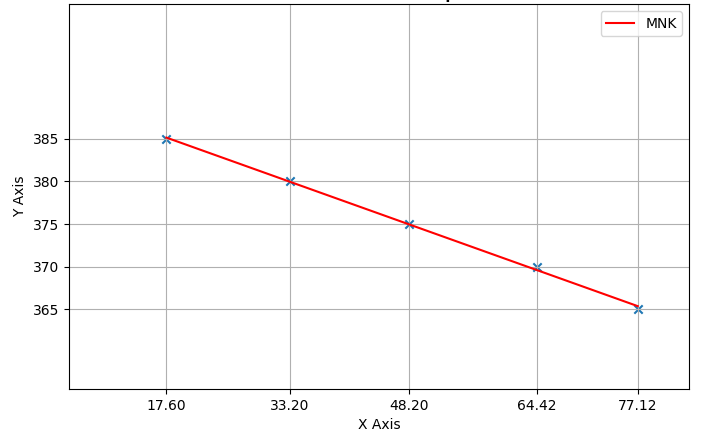
\includegraphics[width=1\textwidth]{pick4}
    \caption{График частоты от времени}
\end{figure}

Из графика получили $\nu $ = 391 Гц
\end{document}